\documentclass[10pt,aspectratio=169]{beamer}

%================================================
% Theme
%================================================
\usetheme[numbering=fraction,progressbar=frametitle]{metropolis}

%================================================
% Packages
%================================================
\usepackage{amsmath,amssymb}
\usepackage{booktabs}
\usepackage{tikz}
\usetikzlibrary{automata,positioning,arrows.meta}

\usepackage{listings}
\usepackage{xcolor}
\usepackage[useregional]{datetime2}

%================================================
% Metadata
%================================================
\newcommand{\LastCompiled}{\DTMnow}

\title{Theory of Computation}
\subtitle{Lecture 3: Finite-State Machines Are Everywhere}
\author{Sheikh Azizul Hakim\\Lecturer, Department of CSE, BUET}
\date{Last compiled: \LastCompiled}

%================================================
% Listings
%================================================
\lstdefinestyle{code}{
  basicstyle=\ttfamily\small,
  frame=single,
  backgroundcolor=\color{black!4},
  rulecolor=\color{black!20},
  showstringspaces=false
}
\lstset{style=code}

%================================================
\begin{document}

%================================================
\maketitle

%================================================
\begin{frame}[standout]
A finite-state machine remembers the past only through its present state.
\end{frame}

%================================================
\begin{frame}{What Is a State?}

A state is a summary of everything that matters about the past.

\vspace{1em}

Examples:

\begin{itemize}
\item Traffic light
\item Elevator
\item Door lock
\item ATM machine
\item TCP connection
\end{itemize}

\vspace{1em}

Question:

\begin{center}
How much memory do these systems have?
\end{center}

\end{frame}

%================================================
\begin{frame}{Example: Traffic Light}

\begin{center}

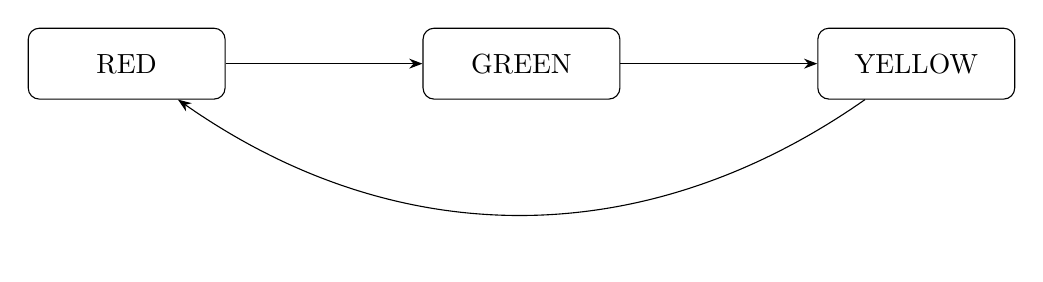
\begin{tikzpicture}[
every node/.style={draw,rounded corners,minimum width=2.5cm,minimum height=0.9cm},
>=Stealth
]

\node (r) {RED};
\node[right=2.5cm of r] (g) {GREEN};
\node[right=2.5cm of g] (y) {YELLOW};

\draw[->] (r) -- (g);
\draw[->] (g) -- (y);
\draw[->] (y) to[bend left=35] (r);

\end{tikzpicture}

\end{center}

\vspace{1em}

The traffic light remembers its history only through its current color.

\end{frame}

%================================================
\begin{frame}{Example: Door Lock}

Possible states:

\[
\texttt{LOCKED}
\qquad
\texttt{UNLOCKED}
\]

\vspace{2em}

Question:

Does the lock remember every button ever pressed?

\pause

No.

It remembers only its current state.

\end{frame}

%================================================
\begin{frame}{Example: Password Validator}

Suppose the PIN is

\[
3141
\]

What information must we remember?

\pause

Possible states:

\begin{itemize}
\item Nothing matched
\item 3 matched
\item 31 matched
\item 314 matched
\item Accepted
\item Dead state
\end{itemize}

\pause

A finite number of situations is sufficient.

\end{frame}

%================================================
\begin{frame}{A State Machine for PIN 3141}

\begin{center}

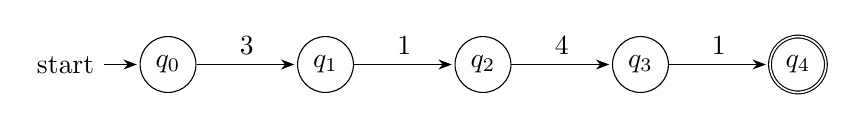
\begin{tikzpicture}[
->,
>=Stealth,
shorten >=1pt,
node distance=2cm,
every state/.style={
minimum size=7mm,
draw
}
]

\node[state,initial] (q0) {$q_0$};
\node[state,right of=q0] (q1) {$q_1$};
\node[state,right of=q1] (q2) {$q_2$};
\node[state,right of=q2] (q3) {$q_3$};
\node[state,accepting,right of=q3] (q4) {$q_4$};

\path
(q0) edge node[above]{3} (q1)
(q1) edge node[above]{1} (q2)
(q2) edge node[above]{4} (q3)
(q3) edge node[above]{1} (q4);

\end{tikzpicture}

\end{center}

We can recognize a pattern by moving between states.

\end{frame}

%================================================
\begin{frame}{Example: Even Number of 1's}

Question:

Does the string

\[
1100101
\]

contain an even number of \(1\)'s?

\pause

What do we need to remember?

\pause

Only two possibilities:

\[
\texttt{EVEN}
\qquad
\texttt{ODD}
\]

\vspace{1em}

We do not need to remember the entire string.

\end{frame}

%================================================
\begin{frame}{A State Machine for Parity}

\begin{center}

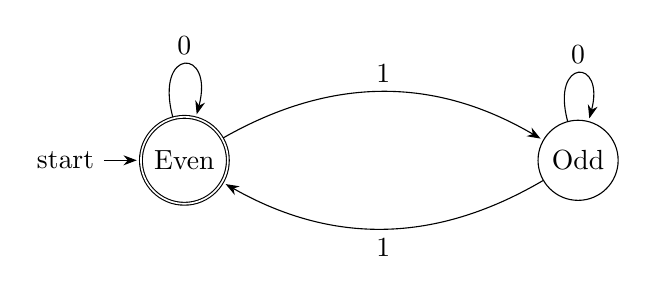
\begin{tikzpicture}[
->,
>=Stealth,
shorten >=1pt,
node distance=5cm,
every state/.style={
minimum size=8mm,
draw
}
]

\node[state,accepting,initial] (e) {Even};
\node[state,right of=e] (o) {Odd};

\path
(e) edge[loop above] node{0} ()
(e) edge[bend left] node[above]{1} (o)
(o) edge[loop above] node{0} ()
(o) edge[bend left] node[below]{1} (e);

\end{tikzpicture}

\end{center}

Only one bit of memory is necessary.

\end{frame}

%================================================
\begin{frame}[fragile]{Example: Compiler Tokenizer}

Input:

\begin{lstlisting}
if (x == 10)
\end{lstlisting}

\vspace{1em}

How does the compiler recognize

\begin{center}
\texttt{if}
\end{center}

as a keyword?

\pause

It moves through a finite number of states:

\[
\texttt{Start}
\rightarrow
\texttt{i}
\rightarrow
\texttt{if}
\]

\pause

Compilers are full of finite-state machines.

\end{frame}

%================================================
\begin{frame}{Example: TCP Connection}

Possible states:

\begin{itemize}
\item LISTEN
\item SYN\_SENT
\item ESTABLISHED
\item FIN\_WAIT
\item CLOSED
\end{itemize}

\vspace{1em}

Operating systems often model communication protocols as state machines.

\end{frame}

%================================================
\begin{frame}{The Big Idea}

Computation proceeds one symbol at a time.

\[
\text{Input}
\rightarrow
\text{Current State}
\rightarrow
\text{New State}
\rightarrow
\cdots
\rightarrow
\text{Accept/Reject}
\]

\vspace{1em}

The machine stores only its current state.

\end{frame}

%================================================
%================================================
\begin{frame}{Can These Be Solved Using Only Finite Memory?}

Suppose a machine reads the input from left to right and can remember
only finitely many states. For each problem, predict:

\begin{center}
\textbf{Can a finite-state machine solve it?}
\end{center}

\begin{enumerate}
\item Does a binary string contain an even number of \(1\)'s?
\pause
\item Does a binary string end with \(001\)?
\pause
\item Is a password valid according to some fixed rules?
\pause
\item Are the parentheses balanced?
\pause
\item Is the number of \(0\)'s equal to the number of \(1\)'s?
\pause
\item Is the input a syntactically valid JSON file?
\end{enumerate}

\vfill

\pause
\begin{center}
\alert{Which of these require only finite memory, and which require more?}
\end{center}

\end{frame}
%================================================
%================================================
\begin{frame}[standout]

Regular Languages

=

Languages recognizable by finite-state machines.

\end{frame}

\begin{frame}[standout]

Next lecture:

Deterministic Finite Automata (DFA)

\[
M=(Q,\Sigma,\delta,q_0,F)
\]

\end{frame}

%================================================
\end{document}

